% !TEX root = ../ac_paper.tex

\section{Introduction\label{sec:intro}}

We live in an extraordinary time where artificial intelligence (AI) is transforming numerous sectors and professions. Recent advancements in Large Language Models (LLMs) have enabled AI to read, write, and converse in over 90 languages, achieving proficiency comparable to human experts. In the realm of board games, AI has surpassed even the best human players. As AI continues to evolve, a critical question is: Can AI systems reason as effectively as humans across various general domains?

Mathematics seems like a very natural step on a path toward Artificial General Intelligence (AGI) due to its universal syntactic and logical structure, akin to natural language. Moreover, mathematics allows for the quantitative evaluation of logical and analytical reasoning, making it an ideal domain for self-improving AI systems on the path to AGI. Momentarily, we will explain yet another reason why mathematics can play a useful role for AGI development, but first we need to introduce one more key element: reinforcement learning (RL).

Machine learning, a subfield of AI, involves developing algorithms and statistical models that enable computers to learn and make predictions from data. Among the three primary areas of machine learning --- supervised learning, unsupervised learning, and reinforcement learning --- RL focuses on learning through interaction with an environment and receiving feedback in the form of rewards or penalties. It is this aspect of machine learning, which can be characterized as having its focus on AI models `playing games,' that will be central to our discussion.

A typical chess game lasts about 30-40 moves, with the longest recorded professional game reaching 269 moves, ending in a draw between Ivan Nikolic and Goran Arsovic in 1989. Note, the number of moves in a typical chess game is relatively consistent, with the longest professional game having only an order of magnitude more steps than the average. Similarly, a typical game of Go involves a few hundred moves, with the longest recorded professional game, played by Go Seigen and Kitani Minoru in 1933, lasting 411 moves.

At first glance, many mathematical problems --- such as proving or disproving conjectures, proving theorems --- can be formulated as games. For example, proving a theorem requires finding a path from the hypothesis to the goal that consists of basic logical steps, e.g. Lean-steps. From the RL perspective, this type of game can be rather complex due to its large action space. On the other hand, finding examples or counterexamples to settle important conjectures may involve only a few basic moves (actions); the case study in this paper will be a good illustration of a problem of this type. In all cases, the problem is basically a search process, and to a large extent the complexity is determined by the size of the action space and the search space.

In addition, in hard research-level mathematics problems one is faced with yet another challenge: the sought-after instance can be so rare and hard to find that the problem can effectively be a search of a needle in a haystack, i.e. it can be a problem with ultra-sparse rewards. For example, in the context of theorem proving, one can think of an extremely hard theorem\footnote{A proxy for such a problem could be the Riemann hypothesis, or any other unsolved Millennium Prize Problem.} that may require a very large number of steps; if there aren't many alternative proofs, finding a small number of very long ones then becomes a search for a needle in a haystack or, depending on preference, a search for a unicorn.\footnote{Similar challenges, though not as critical, arise also in non-research level math problems, see e.g. \cite{peano,trinh2024solving} for recent discussion. On the other hand, in a parallel line of development new benchmarks were proposed in the past couple of years \cite{procgen,NeedleInAHaystack}, which can be useful in such contexts.}

Fortunately, mathematics provides a robust framework for developing and testing new algorithms with adaptive capabilities that `learn how to learn' dynamically. Testing these algorithms on mathematical problems, rather than directly on societal issues like market crash predictions or extreme weather events, offers a risk-free and cost-effective approach. And, the benefits are that hard mathematical problems can be solved and long-standing conjectures can be resolved in the process of implementing this approach.

Our approach to problems of this type involves endowing the RL model with the ability to assess hardness of problems during the training process. First and foremost, this requires a practically useful notion of {\it hardness}, a concept we thoroughly explore. By learning the distribution of problems based on their difficulty, one can augment existing off-the-shelf algorithms with new self-improvement strategies, identifying key features that facilitate solving the most challenging problems.

In this paper, we initiate a systematic implementation of this approach by carefully analyzing the distribution of hardness in potential counterexamples to a long-standing conjecture, the Andrews-Curtis conjecture. As is the case in many other hard problems, one natural measure of hardness is the number of steps an RL agent needs to make. And, what makes the Andrews-Curtis conjecture particularly suitable for our study is that it includes numerous examples that require a hyper-exponential number of steps, offering an effective testbed for exploring the aforementioned questions through the lens of RL, search algorithms, and topological data analysis.

We should emphasize that this entire project was done with relatively modest computational resources that a small academic research group can easily afford. As a result, we put more emphasis on theoretical tools and techniques that, when combined with scaling of computational resources, can lead to further improvements.

While our primary focus is on exploring the distribution of hardness with an eye toward algorithm development, along the way we resolve a particularly intriguing open case (potential counterexample) that has eluded direct mathematical approaches for decades:

\begin{theorem}\label{thm:stableAK3}
    The following potential counterexample introduced by Akbulut and Kirby \cite{Akbulut--Kirby} is stably AC-trivial:
    \[
    \AK(3) = \angles{x, y \mid x^3 = y^{4}, xyx = yxy}.
    \]
\end{theorem}

\noindent
The proof of this theorem is presented in \autoref{sec:stable_ak3}.

The rest of the paper is organized as follows. In \autoref{sec:AC}, we provide an overview of the Andrews--Curtis conjecture, describing the specific version studied in this work. We then apply classical search algorithms to examples in the Miller--Schupp series in \autoref{sec:search}, where we devise a greedy search algorithm that significantly outperforms the widely used breadth-first search algorithm. In \autoref{sec:rl}, we employ reinforcement learning, specifically implementing the Proximal Policy Optimization (PPO) algorithm \cite{schulman2017proximal}, and find that while it performs better than breadth-first search, it does not surpass the greedy search algorithm (see \autoref{fig:performance}). Building on these insights, \autoref{sec:algo} presents several ideas for algorithm development, proposing strategies to mitigate the overwhelming complexity faced by an RL agent in challenging problems. In \autoref{sec:isolated}, we employ topological methods to assess the complexity of presentations. Specifically, we utilize persistent homology to define the \textit{isolation value} of a presentation. This value is infinite for counterexamples to the AC conjecture and serves as a measure of a presentation's resistance to being trivialized. Finally, in \autoref{sec:lm}, we examine the linguistic structure of balanced presentations using a decoder-only Transformer model, observing distinct clusters within the embedding space corresponding to presentations solved and unsolved by the greedy search algorithm.

\begin{figure}
	\centering
	\begin{subfigure}[b]{0.5\textwidth}
		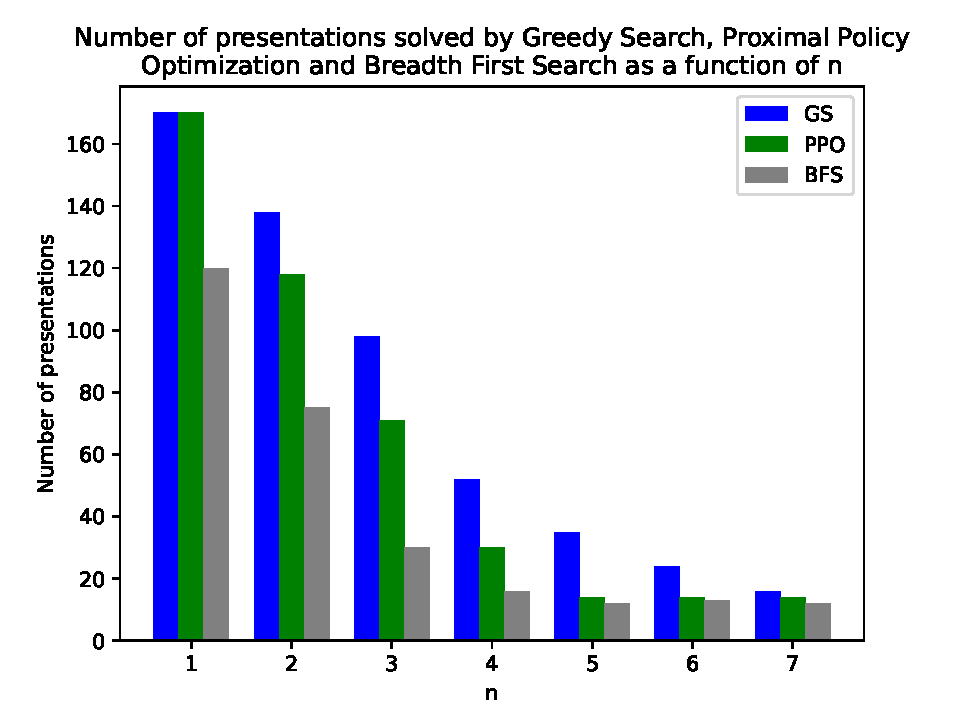
\includegraphics[width=1.1\textwidth]{fig/performance_vs_n.pdf}
		\caption{Distribution versus $n$}
		\label{fig:performance_vs_n}
	\end{subfigure}
	\begin{subfigure}[b]{0.5\textwidth}
		\centering
		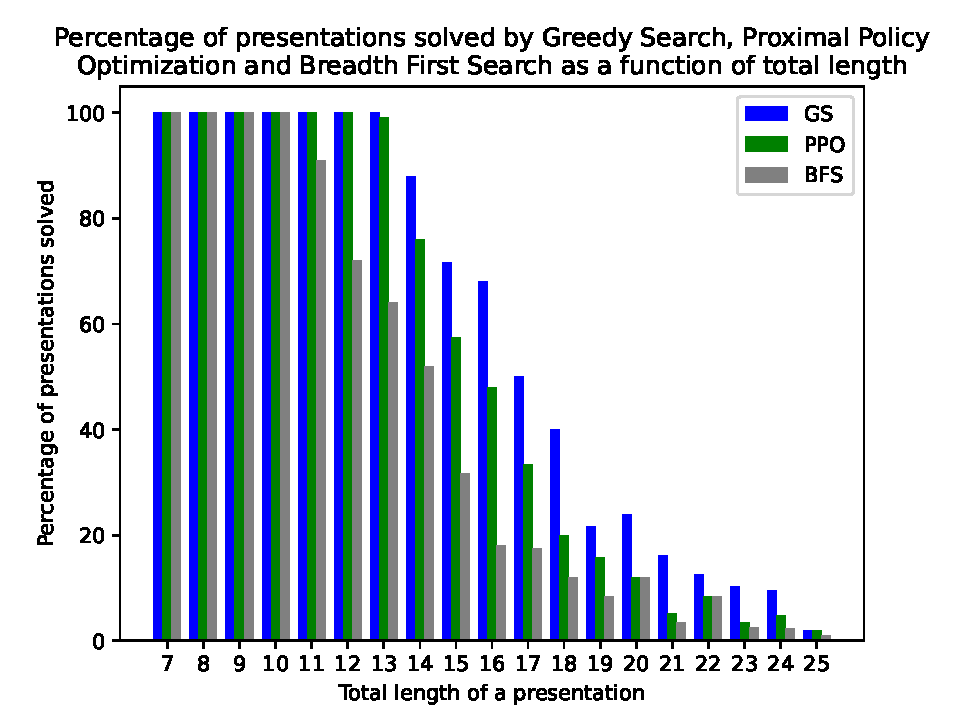
\includegraphics[width=1.1\textwidth]{fig/performance_vs_length.pdf}
		\caption{Distribution versus length}
		\label{fig:performance_vs_length}
	\end{subfigure}
	\caption{A comparison of three algorithms --- breadth-first search, greedy search, and Proximal Policy Optimization (PPO) --- that we used to search through the space of balanced presentations. The number of presentations of the Miller--Schupp series, $\MS(n, w)$, solved by an algorithm is given on the vertical axis. We compare the performance as a function of $n$ (above) and the length of the presentation (below). Greedy Search consistently outperforms Breadth-First Search and Proximal Policy Optimization.}
	\label{fig:performance}
\end{figure}

%We compare the performance of Greedy Search (GS), Breadth First Search and Proximal Policy Optimization on the presentations of Miller--Schupp series with $n, \ \length(w) \leq 7$ in \autoref{fig:performance}.
